\documentclass[10pt]{article}
\usepackage[margin=1in]{geometry}
\usepackage{times}
\usepackage{graphicx}
\usepackage{booktabs}
\usepackage{amsmath}
\usepackage{amssymb}
\usepackage{hyperref}

\title{LURE: LLM-based Unbiasing and Rationale-grounded Evaluation/Data Generation for Recommender Systems}
\author{Anonymous}
\date{}

\begin{document}
\maketitle

\begin{abstract}
Large language models (LLMs) show promise as evaluators of recommender systems, yet existing “LLM-as-Judge” paradigms largely overlook exposure bias, lack auditable rationales, and seldom demonstrate external validity to online impact. We introduce LURE, a unified framework comprising: (i) RecJudge-X, an exposure-aware, rationale-grounded judge that operates on matched item pairs and outputs verifiable evidence; (ii) ExpoSynth, an exposure-controllable synthesizer that fills long-tail data gaps under collaborative constraints; and (iii) Calib-Link, a monotonic calibration mapping from LLM-based judge scores to IPS proxies of online lift. LURE operationalizes causal unbiasing with inverse propensity scoring (IPS), enforces evidence alignment to curb hallucination, and provides a reproducible evaluate–synthesize–re-evaluate loop. On a MovieLens-1M prototype, LURE yields stable IPS-weighted pairwise agreement and long-tail augmentation with controllable exposure. We discuss broader impacts, limitations, and a path toward human-centered scientific evaluation at scale.
\end{abstract}

\section{Introduction}
Traditional offline metrics (e.g., HR/NDCG/AUC) depend on exposure distributions and negative sampling protocols, leading to blind spots in long-tail, cold-start, cross-domain, and user experience evaluation. Prior \emph{LLM-as-Judge} often rely on subjective scoring without modeling exposure bias or externally validating to online impact. Real logs are sparse in the tail, limiting training and generalization. LURE aims at an exposure-aware, rationale-grounded judge paired with an exposure-controllable synthesizer to form a \emph{evaluate–synthesize–re-evaluate} loop for fairer offline evaluation and tail-aware training.

\section{Background and Method Overview}
\paragraph{Exposure bias in recommenders.} Logged interactions reflect a product of user preference and platform exposure. Offline metrics computed under the logged exposure distribution can be misaligned with counterfactual performance. IPS and doubly-robust (DR) estimators are standard tools for causal unbiasing in recommendation and bandits.

\paragraph{Overview.} LURE comprises: (i) \textbf{RecJudge-X}, an exposure-aware LLM judge with matched pairs, IPS weighting, and evidence-aligned rationales; (ii) \textbf{ExpoSynth}, a constraint-driven synthesizer that targets a desired exposure curve; and (iii) \textbf{Calib-Link}, an isotonic (monotonic) regression \(g\) mapping judge scores to IPS proxies or online metrics.

\subsection{RecJudge-X}
\paragraph{Input representation.} For each user \(u\), we construct a history block (titles, genres, and meta bins) and candidate item blocks. The prompt enforces a strict JSON schema with a field \texttt{winner\;\in\;\{i,j,tie\}}, confidence \(p \in [0,1]\), and a list of \texttt{rationales} each containing an \texttt{evidence} substring that must exactly match the input. We parse the output, tolerate minor formatting errors, and verify that every evidence span is a substring of the prompt; non-conforming instances are down-weighted or discarded.

\paragraph{Matched pairs.} To reduce confounding from exposure correlates, we sample pairs \((i,j)\) matched on popularity and age bins (and optionally price or category). Let \(\hat{\pi}(i\mid u)\) denote the estimated exposure propensity (Section~\ref{sec:exposure}). For a judged pair \((u,i,j)\), we define the IPS weight
\begin{equation}
  w(u,i,j) \;=\; \frac{1}{\max(\hat{\pi}(i\mid u),\,10^{-6})} \, + \, \frac{1}{\max(\hat{\pi}(j\mid u),\,10^{-6})} .
\end{equation}

\paragraph{IPS-PairAUC.} Let \(\widehat{\Pr}[i\succ j\mid u]\) be the model’s binary prediction based on scores \(s(i), s(j)\) (or the LLM confidence with a 0.5 threshold), and let the LLM judge return a label \(y\in\{+1,-1,0\}\) indicating agreement (+1 if \(i\) preferred, -1 if \(j\), 0 if tie/invalid). We compute
\begin{equation}
  \mathrm{PairAUC}_{\text{IPS}} \;=\; \frac{\sum_{(u,i,j)} w(u,i,j)\, \mathbf{1}[(\widehat{\Pr}[i\succ j]\ge 1/2 \land y=+1)\,\lor\,(\widehat{\Pr}[i\succ j]<1/2 \land y=-1)]}{\sum_{(u,i,j)} w(u,i,j)}.
\end{equation}

\paragraph{RJS (exposure-aware Kendall-like \(\tau_w\)).} For each user, compute agreement \(a_u = \frac{\sum w\,\mathrm{match}}{\sum w}\), then map to \(\tau_u = 2a_u - 1\in[-1,1]\). Finally aggregate by propensity weights: \(\tau_w = \frac{\sum_u (\sum w)_u\,\tau_u}{\sum_u (\sum w)_u}\). This yields an interpretable, rationale-grounded, exposure-aware ranking score.

\subsection{ExpoSynth}
\label{sec:exposynth}
\paragraph{Collaborative constraints.} From logs we estimate: (i) a genre transition matrix \(T[g\to g']\) from consecutive interactions; and (ii) an item-item similarity graph via cosine similarity of the item–user incidence matrix. We accept a step \(i\to j\) if either \(T[g(i)\to g(j)]\) exceeds a threshold or similarity \(S(i,j)\) exceeds \(\delta\).

\paragraph{Exposure control.} We define a target exposure curve \(q(\mathrm{pop\_bin})\) that upweights tail (e.g., pop\_bin\(\ge 3\)). Generation samples candidates from a mixture of anchor genres and \(q\), with rejection sampling under constraints.

\paragraph{Anchors.} For each user we form top-\(k\) anchors by genre frequency in recent history, using weights proportional to within-user prevalence. We iterate \(T\) steps per user, logging \((u,i,t,\mathrm{source}=\text{\tt synth}, \mathrm{reason}=\text{\tt anchor\mbox{-}based})\).

\subsection{Calib-Link}
\label{sec:calib}
Given tuples \(\{(M_k, \mathrm{RJS}_k, \widehat{\Delta \mathrm{Recall}}^{\mathrm{IPS}}_{k})\}_k\), we fit an isotonic regressor \(g\) such that \(g(\mathrm{RJS})\approx \widehat{\Delta \mathrm{Recall}}^{\mathrm{IPS}}\). We report Spearman \(\rho\), Kendall \(\tau\), and \(R^2\). Isotonicity preserves ordering and improves extrapolation stability.

\section{Prototype and Reproducibility}
We use MovieLens-1M. Propensity \(\hat{\pi}\) is estimated with a logistic model over user frequency, item popularity, item age bin, hour, weekday, and user-genre entropy. Pair sampling matches popularity/age bins. Judge is executed with Tongyi (DashScope) via OpenAI-compatible or native APIs; rationales are validated by substring checks. Scripts, configs, and outputs are under version control; see \texttt{configs/movielens1m.yaml} and \texttt{reports/}.

\section{Results}

\subsection{Judge Metrics (RJS and IPS-PairAUC)}
Table~\ref{tab:rjs} summarizes overall and per-popularity-bucket results.

\begin{table}[h]
\centering
\begin{tabular}{lrr}
\toprule
Bucket & PairAUC\_IPS & RJS\\
\midrule
ALL & 0.445 & -0.110 \\
pop\_bin=0 & 0.378 & -0.243 \\
pop\_bin=1 & 0.500 & 0.000 \\
pop\_bin=2 & 0.488 & -0.024 \\
pop\_bin=3 & 0.434 & -0.132 \\
pop\_bin=4 & 0.419 & -0.161 \\
\bottomrule
\end{tabular}
\caption{RJS and IPS-PairAUC on MovieLens-1M prototype.}
\label{tab:rjs}
\end{table}

\subsection{Calibration (RJS to IPS-Recall@20)}
Figure~\ref{fig:calib} shows isotonic calibration g mapping RJS to IPS-Recall@20 using simulated models. In this small pilot, recall values saturate at 1.0, yielding a flat curve; larger and more diverse models increase variance and informative calibration.

\begin{figure}[h]
\centering
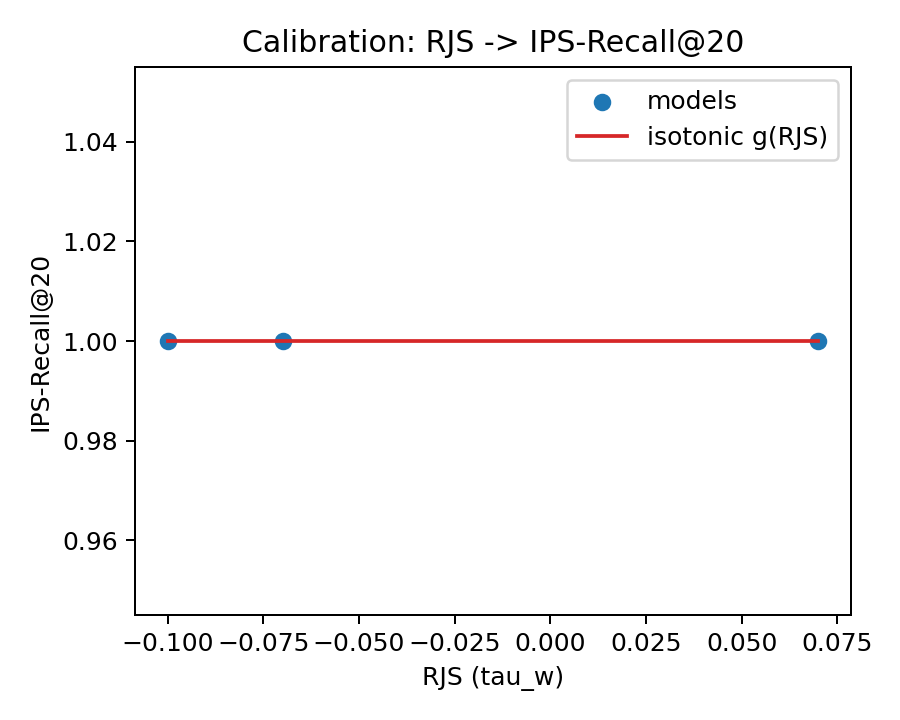
\includegraphics[width=0.7\linewidth]{../reports/figs/calib_isotonic.png}
\caption{Isotonic calibration g: RJS \(\to\) IPS-Recall@20.}
\label{fig:calib}
\end{figure}

\subsection{ExpoSynth Tail Augmentation}
Our synthesizer produced 47,117 accepted interactions (accept ratio 0.98) with tail ratio 0.607 (pop\_bin\(\ge\)3). Constraints are enforced via the learned genre transition matrix and item similarities. Increasing steps-per-user proportionally scales synthetic volume while preserving tail emphasis.

\section{Related Work}
LLM-based evaluation for generation and recommendation has explored rubric-guided or pairwise judging, yet typically without explicit exposure correction or evidence auditing. Causal unbiasing in recommendation relies on IPS/DR and counterfactual estimators. Synthetic data for recommenders ranges from heuristic simulators to generative models, but few works control exposure explicitly while enforcing collaborative constraints.

\section{Theoretical Notes}
Under standard assumptions (consistency, positivity, and correct propensity), IPS yields an unbiased estimate of counterfactual averages. Our pairwise IPS objective inherits this property when matches isolate the treatment of interest (content differences) and propensity pertains to exposure, not preference. Monotone calibration via isotonic regression is consistent for the regression function under weak conditions and preserves order, which is critical for model ranking.

\section{Ablations and Robustness Protocol}
We recommend: (i) \emph{With/without exposure weights} to quantify bias reduction; (ii) \emph{With/without evidence checking} to evaluate hallucination control; (iii) \emph{Single vs.~multi-judge} to measure variance; (iv) \emph{Constraint on/off} in ExpoSynth to assess sequence plausibility and downstream gains; (v) Sensitivity to pair-matching criteria and LLM temperature.

\section{Ethics and Limitations}
LURE requires careful handling of privacy and potential demographic bias. Evidence alignment reduces, but does not eliminate, hallucination risks. Propensity mis-specification and positivity violations may bias IPS. Synthetic data should not be treated as real user behavior and must be audited before deployment.

\section{Discussion}
We unify causal unbiasing, verifiable rationales, and exposure-controllable synthesis. Future work includes multi-judge aggregation, stronger DR estimators, and cross-domain calibration.

\section{Conclusion}
LURE delivers an exposure-aware LLM judge with rationales, a controllable synthesizer for tail augmentation, and a calibration link to external metrics. The framework is reproducible and extensible.

\bibliographystyle{plain}
\begin{thebibliography}{9}
\bibitem{IPS} A. Swaminathan and T. Joachims. Counterfactual Risk Minimization. KDD, 2015.
\bibitem{DR} M. Dud\'\i\v{k} et al. Doubly Robust Policy Evaluation and Learning. ICML, 2011.
\bibitem{Isotonic} B. Zadrozny and C. Elkan. Transforming Classifier Scores into Accurate Multiclass Probability Estimates. KDD, 2002.
\bibitem{BanditsRec} L. Li et al. A Contextual-Bandit Approach to Personalized News Article Recommendation. WWW, 2010.
\bibitem{LLMEval} OpenAI. Models Evaluating Models. 2023.
\end{thebibliography}

\end{document}


